\documentclass{article}
\usepackage[preprint]{neurips_2026}

\usepackage[utf8]{inputenc}
\usepackage[T1]{fontenc}
\usepackage{hyperref}
\usepackage{url}
\usepackage{booktabs}
\usepackage{amsfonts}
\usepackage{amsmath}
\usepackage{amssymb}
\usepackage{graphicx}
\usepackage{multirow}
\usepackage{xcolor}

\title{Do Better Imagined Rollouts Mean Better Robot Control? A Controlled Study of World-Model Evaluation Under Feedback}

\author{
  Dharini Raghavan, Amritpal Singh \\
  Georgia Institute of Technology, Emory University 
}

\begin{document}

\maketitle

\begin{abstract}
Robot world models are increasingly used to predict the consequences of actions, train policies in imagination, and evaluate behavior before real-world deployment. This makes rollout fidelity an appealing evaluation target. But robot control is usually closed loop: the robot acts, observes again, updates its internal state, and replans. In this work, we ask whether a model that predicts better when rolled forward without new observations also produces better closed-loop control. We study this question in a small testbed that isolates prediction from perception. We simulate a differential-drive robot that tracks a path under biased odometry and intermittent landmark sensing. We compare six predictive state estimators across 24 sensing conditions and score each one by ordinary replay error, a 20-step measurement-free rollout, and closed-loop tracking error. The rollout metric is the weaker deployment proxy: its Spearman correlation with closed-loop cross-track RMSE is $0.774$, compared with $0.923$ for replay position RMSE, and it selects the wrong closed-loop winner in 18/24 conditions. We then train three learned estimators on much longer synthetic sensing blackouts. The added rollout exposure helps the EKF-anchored models under compound stress, including a reduction in GRU-EKF tracking RMSE from $1.72$ to $1.06$ m, but gives no consistent gain under isolated blackouts and does not help the dead-reckoning-anchored model. These results point to a practical requirement for robot world-model benchmarks: prediction should be evaluated under the same observation and replanning pattern in which the model will be used. Long-horizon fidelity is useful, but it is not a substitute for measuring closed-loop utility. Code and results are available at \url{https://github.com/rdharini2001/Selective-State-Space-Observers-for-Estimate-Driven-Robot-Control-Under-Intermittent-Sensing}.
\end{abstract}

\paragraph{Keywords.} world models; robot learning; imagined rollouts; closed-loop control; world-model evaluation; physical AI.

\section{Introduction}

World models are becoming part of the control stack for physical agents. Recent systems use large video or latent dynamics models to generate possible futures, evaluate robot policies, or produce actions directly from learned spatiotemporal dynamics \citep{agarwal2025cosmos,gemini2025veo,ye2026dreamzero,kim2026cosmospolicy}. This progress raises an evaluation question that is easy to state and hard to answer: what property of a predicted future tells us that the model will be useful for control?

The usual answer is some form of predictive fidelity. A model is judged by reconstruction error, next-state error, perceptual quality, or consistency over a rollout. These scores are important. A model that ignores physical dynamics is unlikely to support reliable control. But fidelity and control utility are not the same quantity. A controller does not simply inspect a prediction; it acts on it. That action changes the next state, a new observation may arrive, the model may be corrected, and the process repeats. An offline metric can therefore rank two models differently from the closed-loop system that actually uses them.

This distinction is especially relevant to imagined rollouts. A long open-loop rollout looks closer to model-based planning than a one-step prediction does, so it is natural to expect it to be a better evaluation metric. Yet many robots do not operate open loop for long periods. They reobserve, update, and replan. A metric that removes future observations may test extrapolation well while testing the deployed feedback loop poorly.

Directly separating these effects in current video world models is difficult. Representation quality, dynamics, action conditioning, policy quality, observation frequency, and replanning are all entangled, and large sweeps are expensive. We therefore use a smaller system in which these factors can be controlled. A differential-drive robot tracks a known path while odometry is biased and range-bearing measurements arrive intermittently. The controller acts on an estimated pose rather than the true pose, so prediction error immediately enters the control loop.

We treat the estimator as a minimal predictive state model. It consumes motion inputs and observations, carries an internal state through time, predicts the robot state, and can be rolled forward after observations are removed. By stripping away image generation and representation learning, the testbed isolates one question that also appears in larger world-model systems: how should offline predictive accuracy be related to downstream control when the model is periodically reconditioned on new information?

We compare dead reckoning (DR), an extended Kalman filter (EKF), and four learned residual observers built on DR or the EKF. Across 24 controlled sensing conditions, each model is evaluated in three ways: replay on logged trajectories, a 20-step measurement-free rollout from a copied internal state, and closed-loop path tracking. Replay position RMSE is more closely aligned with closed-loop control than the longer blind rollout: Spearman $\rho=0.923$ versus $0.774$, with 5/24 versus 18/24 wrong model selections.

We also ask the corresponding training question. Three learned observers are retrained with synthetic sensing blackouts substantially longer than those in the standard training set. This helps both EKF-anchored models when several sensing errors occur together, but the benefit does not transfer cleanly to an isolated blackout sweep. One model improves only at the longest blackouts; another becomes worse throughout the sweep. The DR-anchored model does not improve under compound stress.

The paper makes three points for robot world-model evaluation:
\begin{enumerate}
    \item \textbf{A rollout metric can be less useful than a simpler metric when its information pattern does not match deployment.} In our setting, removing all future observations for 20 steps makes the evaluation less predictive of closed-loop control.
    \item \textbf{Training on harder imagined rollouts is not automatically a closed-loop improvement.} Its effect depends on the model architecture, the analytic anchor, and the stress regime.
    \item \textbf{World-model benchmarks should measure fidelity together with feedback-aware utility.} Observation frequency, reconditioning, and replanning are part of the evaluation protocol.
\end{enumerate}

The goal is not to argue that single-step error is generally superior to multi-step prediction. The result is a controlled counterexample to that generalization. It shows why a world-model metric should be tested against the way the model will actually interact with a robot.

\section{Related work}

\textbf{World models for robot learning and evaluation.} World models learn predictive dynamics that can be rolled forward to support planning or policy learning \citep{ha2018worldmodels}. Dreamer makes imagined latent trajectories central to behavior learning \citep{hafner2019dreamer,hafner2023dreamerv3}. More recent physical-AI systems scale predictive modeling to video and action. Cosmos develops video world foundation models for physical AI \citep{agarwal2025cosmos}; DreamZero treats a world-action model as a zero-shot robot policy \citep{ye2026dreamzero}; and Cosmos Policy adapts a video model for visuomotor control and planning \citep{kim2026cosmospolicy}. Generative world models are also being used as evaluation environments: the Gemini Robotics evaluation system uses an action-conditioned video simulator to compare policy performance across nominal and out-of-distribution conditions \citep{gemini2025veo}. These systems make the quality of imagined futures consequential, but they also make clear that prediction is embedded in a larger loop of action, observation, and replanning.

\textbf{Prediction quality versus decision quality.} Model-based control has long faced an objective mismatch between fitting dynamics and producing good decisions. Lambert et al. \citep{lambert2020objective} show that lower model error need not yield a better model-based RL policy. Our study isolates the same issue at the state-estimation interface. Instead of changing a learned dynamics model and retraining a policy, we place different predictive estimators inside the same controller and directly measure how offline model rankings transfer to closed-loop behavior.

\textbf{Hybrid state estimation.} The EKF remains a standard tool for nonlinear localization with known motion and measurement models \citep{thrun2005probabilistic}. Learned estimators often retain analytic structure while learning uncertain components, including Backprop KF \citep{ha2016backprop}, deep variational Bayes filters \citep{karl2017dvbf}, recurrent Kalman networks \citep{becker2019rkn}, differentiable particle filters \citep{jonschkowski2018dpf}, latent ODEs \citep{rubanova2019latentode}, and KalmanNet \citep{revach2022kalmannet}. Our residual observers follow this hybrid design. The comparison between DR and EKF anchors also lets us test whether rollout training can compensate for a weak underlying state estimate.

\section{Controlled testbed}
\label{sec:system}

The robot state is $s_t=(x_t,y_t,\theta_t)$ and follows unicycle dynamics with $\Delta t=0.1$ s. A pure-pursuit controller with look-ahead distance $L_d=0.8$ m tracks a lemniscate reference path. Odometry is corrupted by multiplicative wheel slip and additive gyroscope bias. The robot also receives range-bearing observations to a fixed landmark map. Sensing degrades in four controlled ways: increased range noise, fewer active landmarks, gyroscope bias, and scheduled intervals in which all landmark measurements are removed.

The controller never sees the true pose. It acts on the observer estimate. An estimation error therefore changes the next control input, which changes the future trajectory. This feedback is the main reason the testbed is useful here: the offline prediction objective and the deployed control objective are related but not identical.

\subsection{Predictive state models}

\textbf{Dead reckoning and EKF.} DR integrates odometry without measurement correction. The EKF uses the unicycle motion model and analytic range-bearing Jacobians. It predicts between measurements and updates whenever a landmark observation is available.

\textbf{Learned residual observers.} Each learned observer uses DR or the EKF as an anchor. A recurrent model predicts a residual $r_t$ with either a GRU or a selective diagonal state-space model (SSM) \citep{gu2022s4,gu2024mamba}. The pose estimate is
\[
    \hat{s}_t = \bar{s}_t \oplus r_t,
\]
where $\bar{s}_t$ is the anchor estimate. The six core candidates are DR, EKF, GRU-DR, SSM-DR, GRU-EKF, and SSM-EKF. The learned models are trained by backpropagation through time on 200 domain-randomized expert trajectories.

\textbf{Long-blackout training.} We train a second copy of SSM-EKF, GRU-EKF, and SSM-DR, denoted by $\dagger$. These models use 300 training trajectories; half include one additional synthetic measurement blackout lasting 32--58 steps, compared with 6--27 steps in the standard data. Architecture, loss, and optimizer are unchanged. Sensing does not affect the simulated plant dynamics or odometry stream, so masking the measurement channels creates a valid counterfactual blackout while holding the underlying motion fixed.

\section{Three ways to score the same model}
\label{sec:evaluation}

The experiments compare three evaluation modes that differ mainly in what information the model receives after time $t$.

\textbf{Replay: predict with normal correction.} Each observer processes the same logged trajectory, including odometry, landmark measurements, and measurement masks. We report position and heading RMSE against the true pose. This is the conventional offline estimate of state-prediction accuracy in the testbed.

\textbf{Blind rollout: predict without future observations.} We replay a trajectory through an observer, copy its internal state at regular checkpoints, and roll the copy forward for $H=20$ steps using only the realized odometry sequence. No landmark measurements are provided during the rollout. We report position RMSE at the full horizon, aggregated over checkpoints and ten seeds. This probe asks how quickly the model drifts when it must continue from its current internal state without correction.

\textbf{Closed loop: predict, act, observe, and correct.} The observer runs inside the simulator and its pose estimate drives the pure-pursuit controller. We report cross-track RMSE as the main downstream metric, together with control effort, blackout-recovery time, and divergence fraction.

These modes test different information patterns. Replay repeatedly allows measurements to correct the estimate. The blind rollout removes that correction for two seconds. Closed-loop control also receives intermittent measurements, but prediction errors additionally affect future actions. Our main question is which offline score best predicts the model ranking in this third setting.

For each of 24 sensing conditions, every offline metric selects one of the six core observers. We compare that choice with the observer that obtains the lowest closed-loop cross-track RMSE in the same condition. We report Spearman rank correlation over all 144 observer-condition pairs, the number of conditions in which an offline score chooses the wrong winner, and regret relative to the closed-loop oracle.

\section{Results}

\subsection{The analytic anchor dominates nominal stability}
\label{sec:baseline-results}

\begin{table}[t]
\centering
\small
\caption{Nominal performance, mean over ten seeds. The learned models benefit much more from the EKF anchor than from recurrence alone.}
\label{tab:nominal}
\begin{tabular}{lccc}
\toprule
Observer & Replay pos. RMSE (m) & Cross-track RMSE (m) & Divergence fraction \\
\midrule
DR             & 1.503 & 1.045 & 0.260 \\
EKF            & 0.140 & 0.212 & 0.004 \\
GRU-DR         & 0.281 & 0.694 & 0.140 \\
SSM-DR         & 0.325 & 0.909 & 0.196 \\
GRU-EKF        & \textbf{0.094} & \textbf{0.163} & 0.000 \\
SSM-EKF        & 0.121 & 0.199 & 0.000 \\
\bottomrule
\end{tabular}
\end{table}

Table~\ref{tab:nominal} gives the nominal condition. GRU-EKF has the lowest replay and tracking error, and both EKF-anchored learned observers are substantially more stable than their DR-anchored counterparts. Figure~\ref{fig:sweeps} shows the full degradation sweeps. The best observer changes with sensing quality, but the EKF anchor remains the most reliable source of stability. Under the longest blackouts, the plain EKF can overtake the learned EKF residual models because there is no new measurement information for the learned correction to exploit.

\begin{figure}[t]
\centering
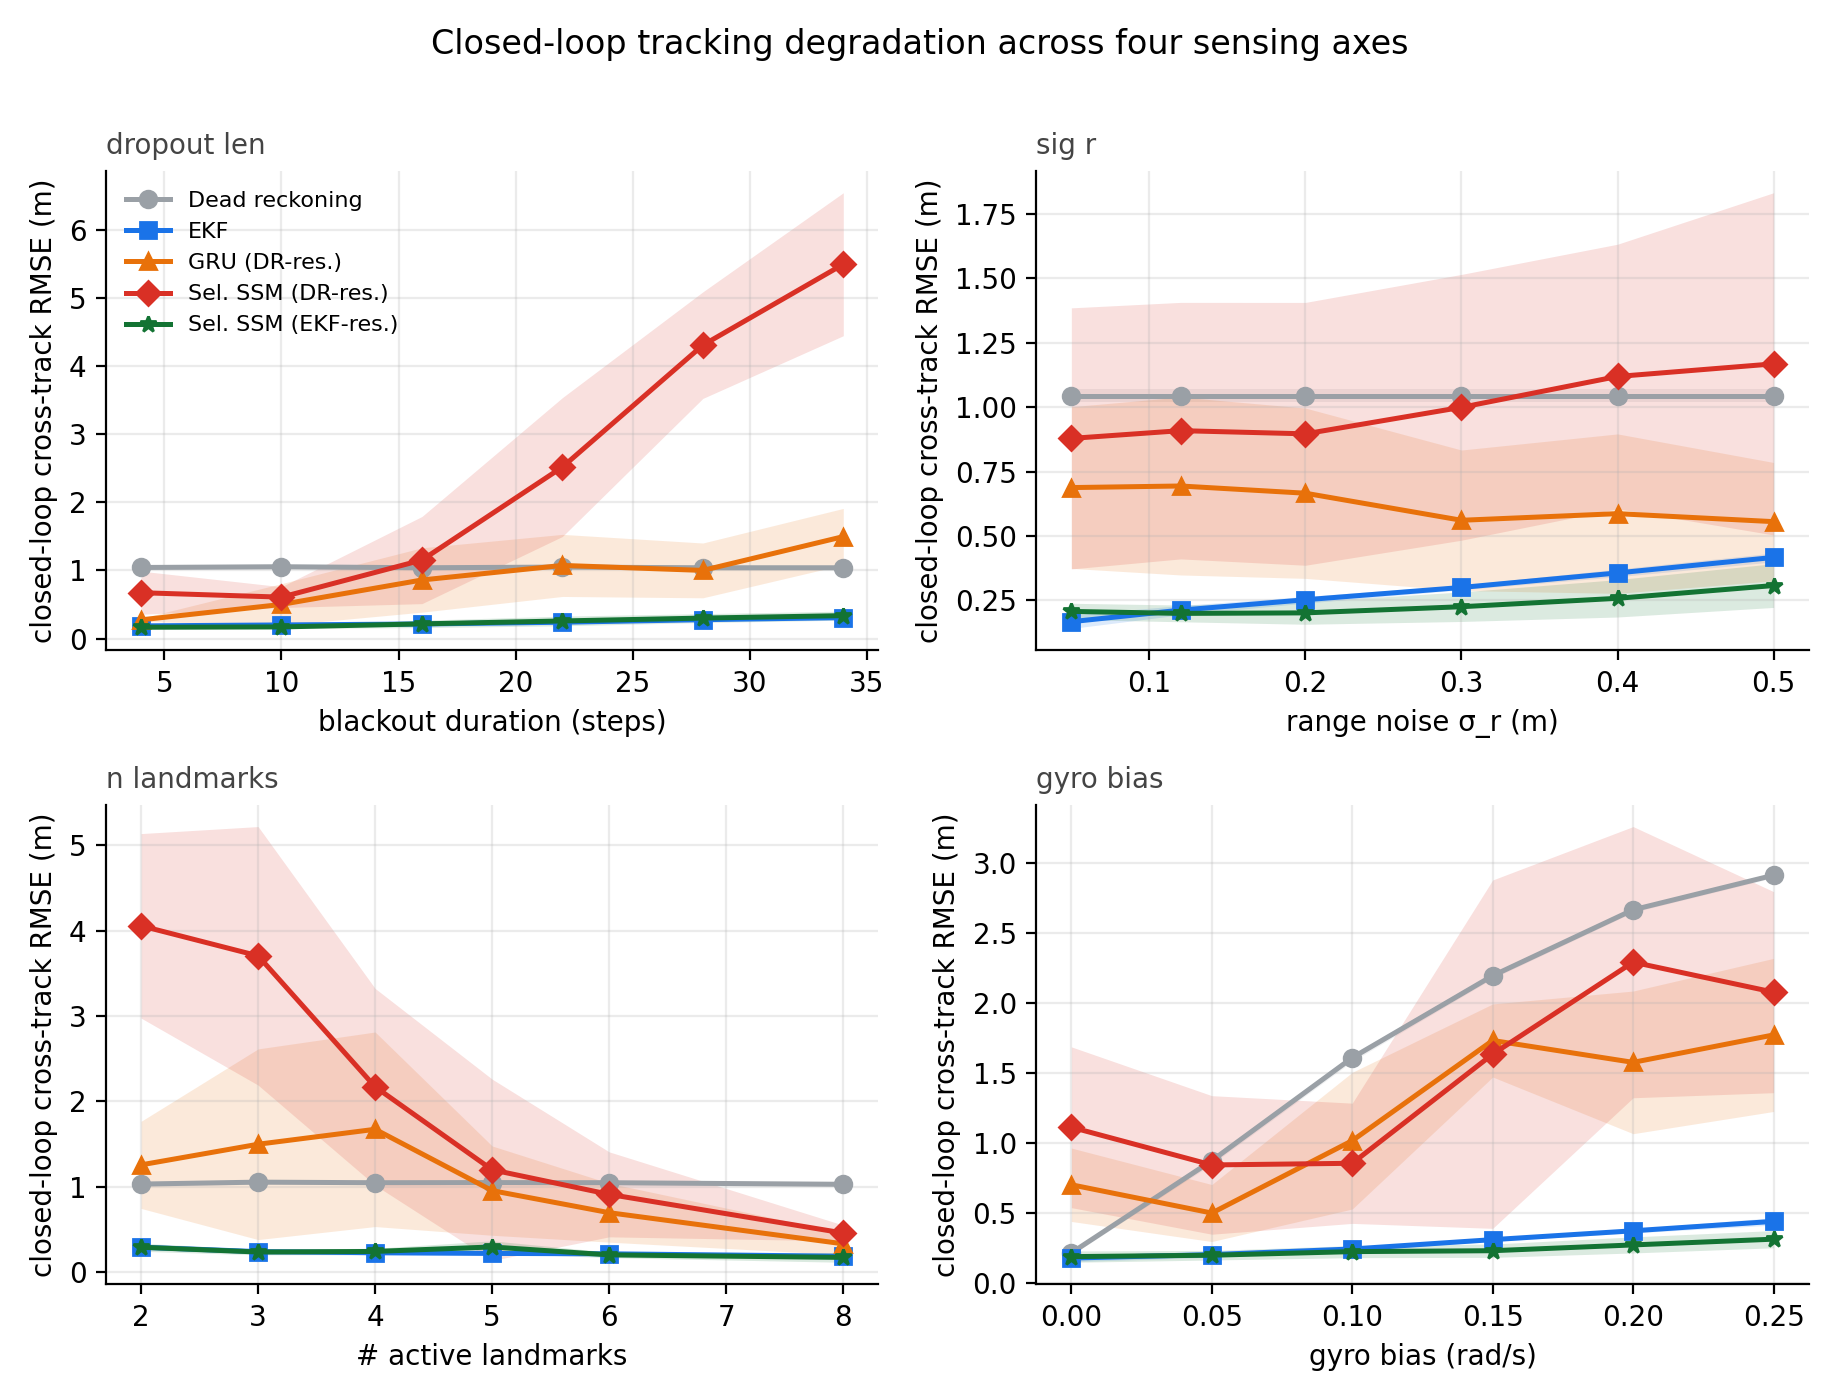
\includegraphics[width=0.92\linewidth]{figures/fig_sweeps.png}
\caption{Closed-loop cross-track RMSE across four sensing-degradation axes. The winner changes with the sensing regime, but EKF-anchored models remain the stable group across the sweep.}
\label{fig:sweeps}
\end{figure}

Across all 144 observer-condition pairs, replay position RMSE and closed-loop cross-track RMSE have Spearman correlation $\rho=0.923$. The relation is strong but not exact: replay position RMSE still selects a different closed-loop winner in 5 of the 24 conditions. This already shows that state-prediction accuracy is an imperfect stand-in for behavior, even before we consider longer imagined rollouts.

\subsection{A longer blind rollout is a worse deployment proxy}
\label{sec:imagination}

A natural expectation is that the 20-step rollout should align better with control than one-step replay because it tests the model in a mode closer to planning. The data do not support that expectation in this feedback setting.

\begin{table}[t]
\centering
\small
\caption{Offline selection criteria across the same 24 conditions and six observers. Higher rank correlation is better; lower failure and regret are better.}
\label{tab:selection}
\begin{tabular}{lcccc}
\toprule
Offline score & Spearman $\rho$ & Top-1 failures & Mean regret (m) & Max regret (m) \\
\midrule
Position RMSE (replay)        & \textbf{0.923} & \textbf{5/24}  & \textbf{0.0051} & \textbf{0.0347} \\
Heading RMSE (replay)         & 0.881 & 19/24 & 0.0237 & 0.0474 \\
Blind-rollout RMSE, $H{=}20$  & 0.774 & 18/24 & 0.0265 & 0.1208 \\
\bottomrule
\end{tabular}
\end{table}

Table~\ref{tab:selection} gives the model-selection result. Blind-rollout RMSE has lower rank correlation with closed-loop tracking, selects the wrong model in 18 of 24 conditions, and has more than three times the worst-case regret of replay position RMSE. Figure~\ref{fig:proxy-scatter} shows the same mismatch over all observer-condition pairs.

\begin{figure}[t]
\centering
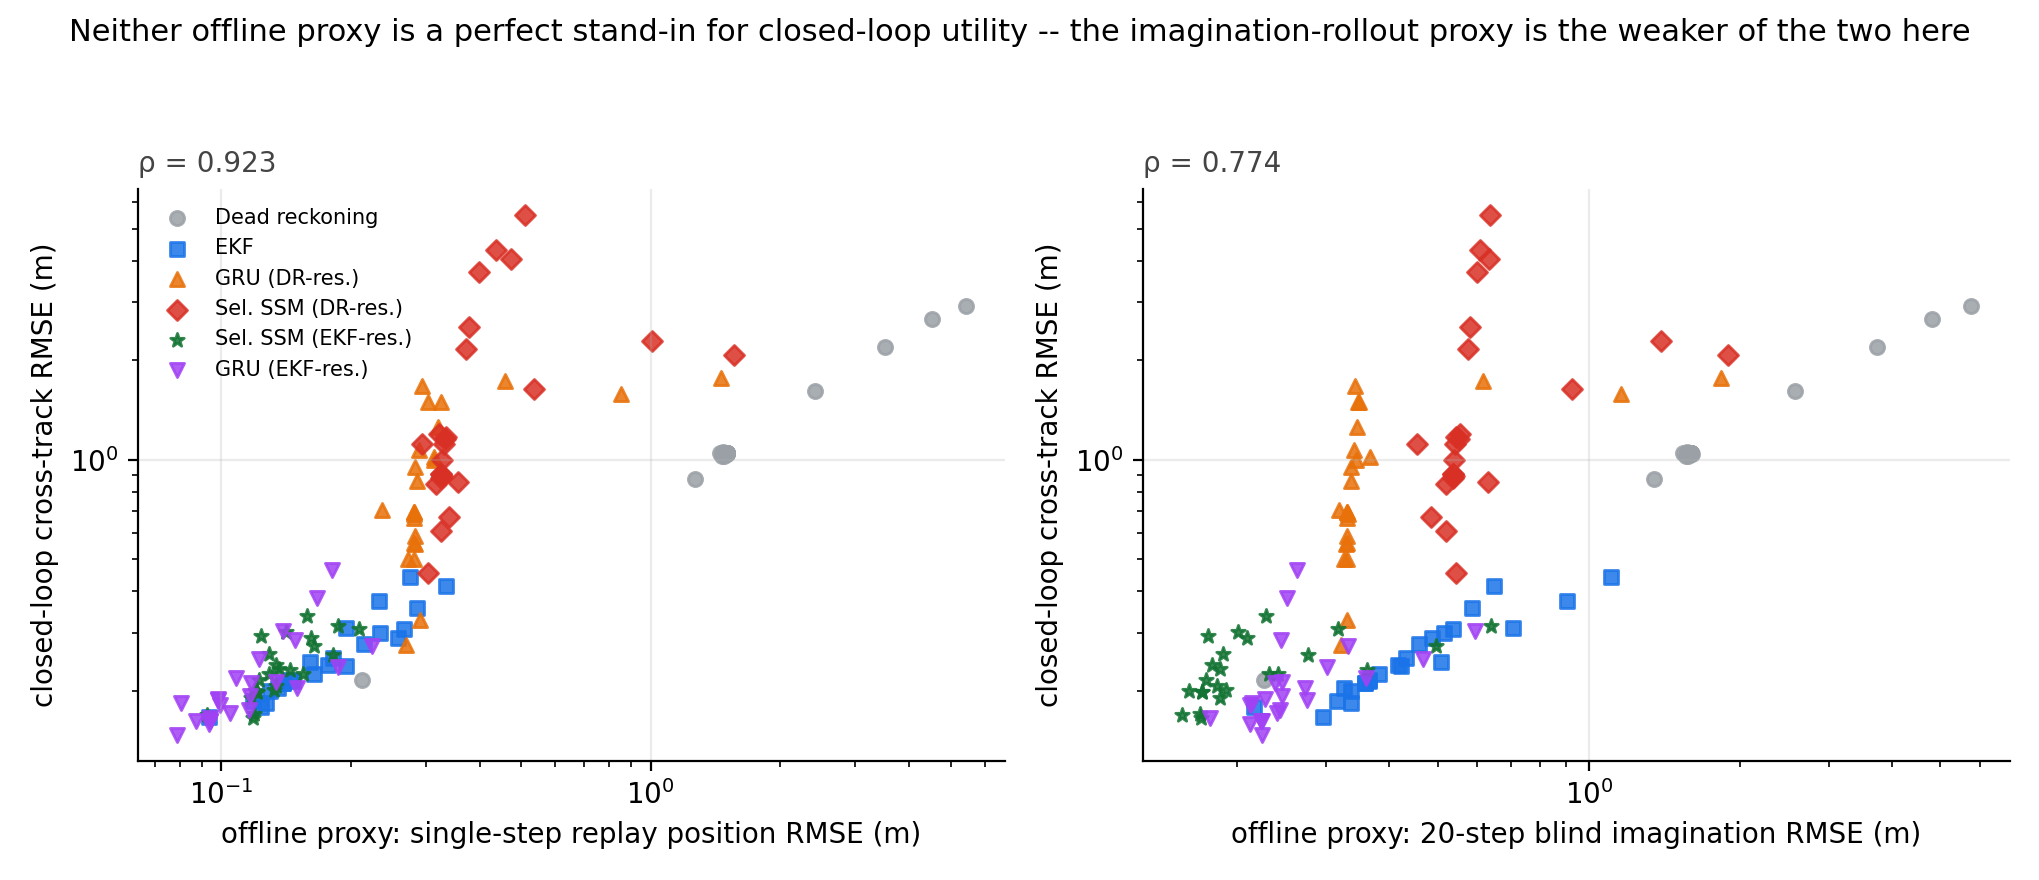
\includegraphics[width=0.98\linewidth]{figures/fig_proxy_scatter.png}
\caption{Closed-loop tracking error versus two offline scores for the same 144 observer-condition pairs. Replay position error (left) tracks closed-loop utility more tightly than the 20-step measurement-free rollout (right).}
\label{fig:proxy-scatter}
\end{figure}

The reason is not that multi-step prediction is meaningless. The two metrics answer different questions. The blind rollout asks: if observations stop now, how accurately can this model extrapolate for two seconds? Closed-loop deployment asks: after prediction, correction, and control are repeatedly interleaved, how well does the robot track the path? An observer can be mediocre at blind extrapolation and still be effective at using the next measurement. A model can also extrapolate well during a blackout yet give a worse corrected estimate over the full trajectory.

Figure~\ref{fig:imagination-growth} makes the distinction visible. Error growth during observation-free prediction differs sharply across models, but that ordering does not reproduce the closed-loop ranking. The important variable is therefore not rollout horizon alone. It is the pair (rollout horizon, observation schedule) that determines how closely the offline probe resembles deployment.

\begin{figure}[t]
\centering
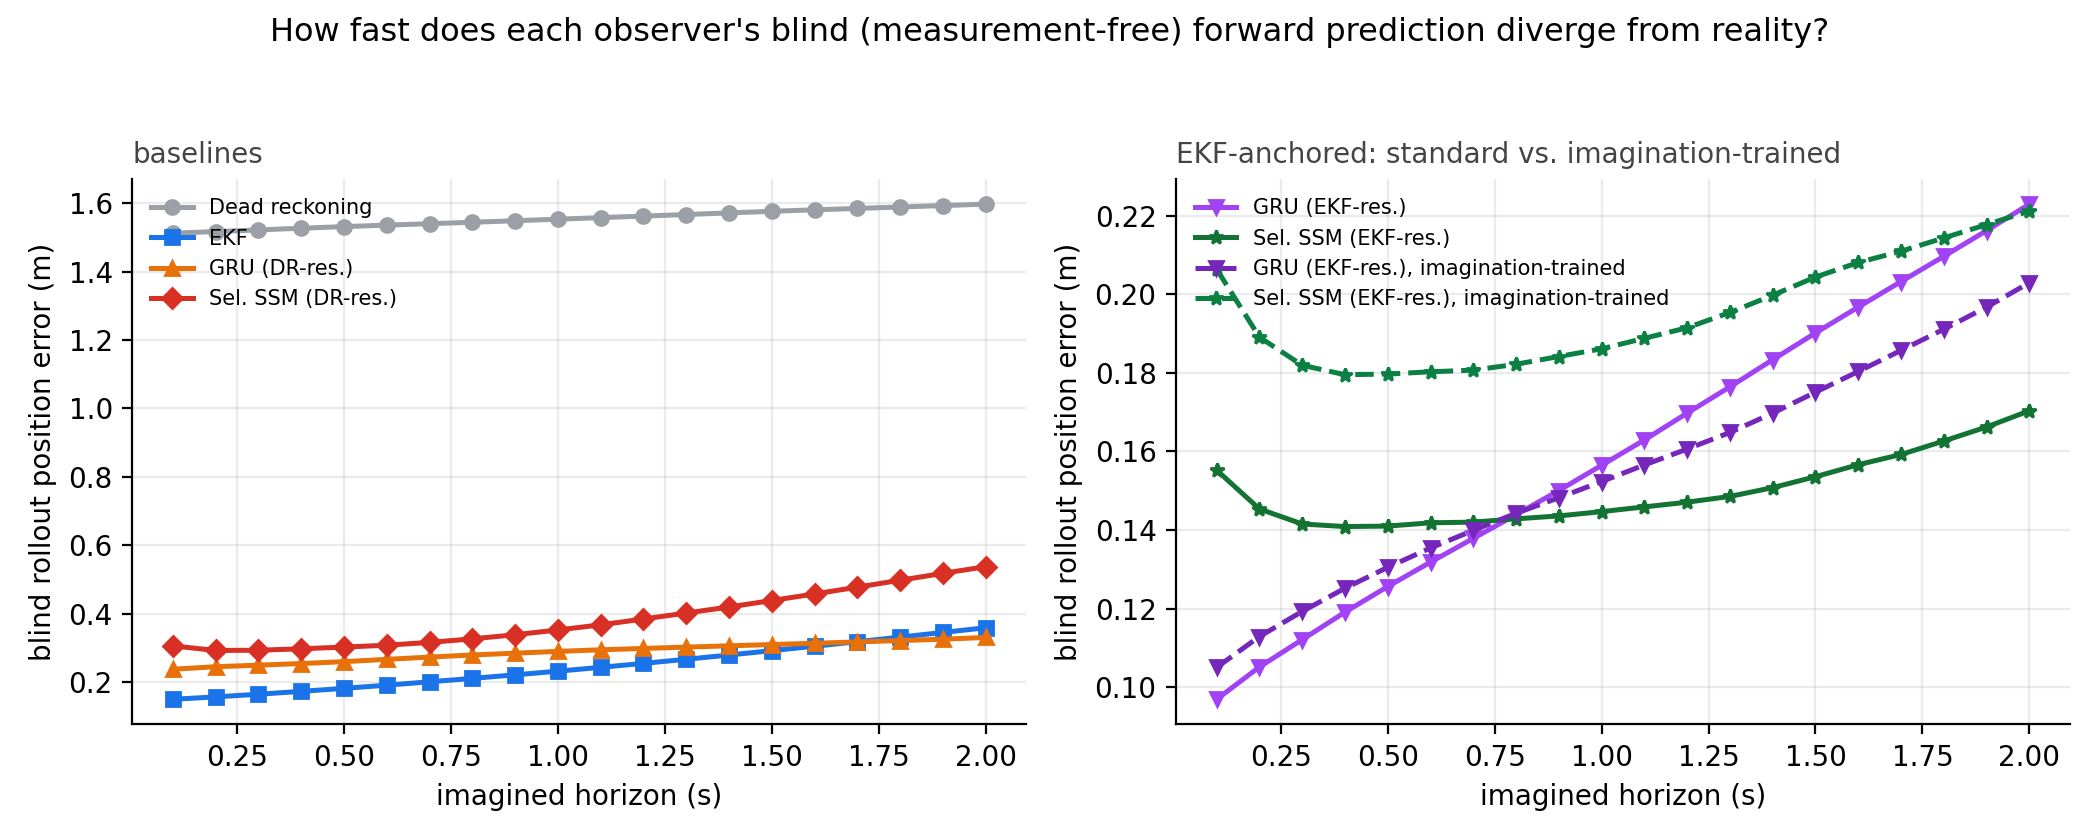
\includegraphics[width=0.90\linewidth]{figures/fig_imagination_growth.png}
\caption{Position error as the observation-free rollout grows in the nominal condition. Left: the six core observers. Right: standard and long-blackout-trained EKF-anchored models. Rollout quality and closed-loop quality need not improve together.}
\label{fig:imagination-growth}
\end{figure}

\subsection{Training on longer blind intervals helps only in some regimes}
\label{sec:curriculum}

The second experiment asks whether long-rollout exposure can improve control even though the blind-rollout metric is not the best model-selection score. We compare the standard and $\dagger$ versions of SSM-EKF, GRU-EKF, and SSM-DR.

\begin{table}[t]
\centering
\small
\caption{Compound stress: high slip, high gyroscope bias, high range noise, a long blackout, and sparse landmarks. Values are means over ten seeds. $\dagger$ denotes long-blackout training.}
\label{tab:compound}
\begin{tabular}{lcc}
\toprule
Observer & Cross-track RMSE (m) & Relative change \\
\midrule
EKF               & 1.800 & -- \\
SSM-EKF           & 1.936 & -- \\
SSM-EKF$^\dagger$ & 1.419 & $-27\%$ \\
GRU-EKF           & 1.717 & -- \\
GRU-EKF$^\dagger$ & \textbf{1.061} & $\mathbf{-38\%}$ \\
SSM-DR            & 5.290 & -- \\
SSM-DR$^\dagger$  & 5.411 & $+2\%$ \\
\bottomrule
\end{tabular}
\end{table}

Under compound stress, longer-blackout training helps both EKF-anchored learned models. SSM-EKF improves from 1.936 to 1.419 m, and GRU-EKF improves from 1.717 to 1.061 m (Table~\ref{tab:compound}). The same training change does not rescue the DR-anchored SSM; its cross-track RMSE increases slightly from 5.290 to 5.411 m.

The isolated blackout sweep tells a different story (Figure~\ref{fig:curriculum}). GRU-EKF$^\dagger$ is close to the standard model over most of the sweep and becomes better only at the two longest blackout settings. At 28 steps, its cross-track RMSE is 0.183 m, compared with 0.286 m for standard GRU-EKF. SSM-EKF$^\dagger$, however, is worse than SSM-EKF at every tested blackout length. The gap grows from 0.233 versus 0.166 m at 4 steps to 0.819 versus 0.336 m at 34 steps. Its blind-rollout RMSE is also higher throughout the sweep, despite being trained on longer blind intervals. Three independent training seeds for SSM-EKF$^\dagger$ preserve the worse long-blackout ordering (Appendix~\ref{app:seeds}).

\begin{figure}[t]
\centering
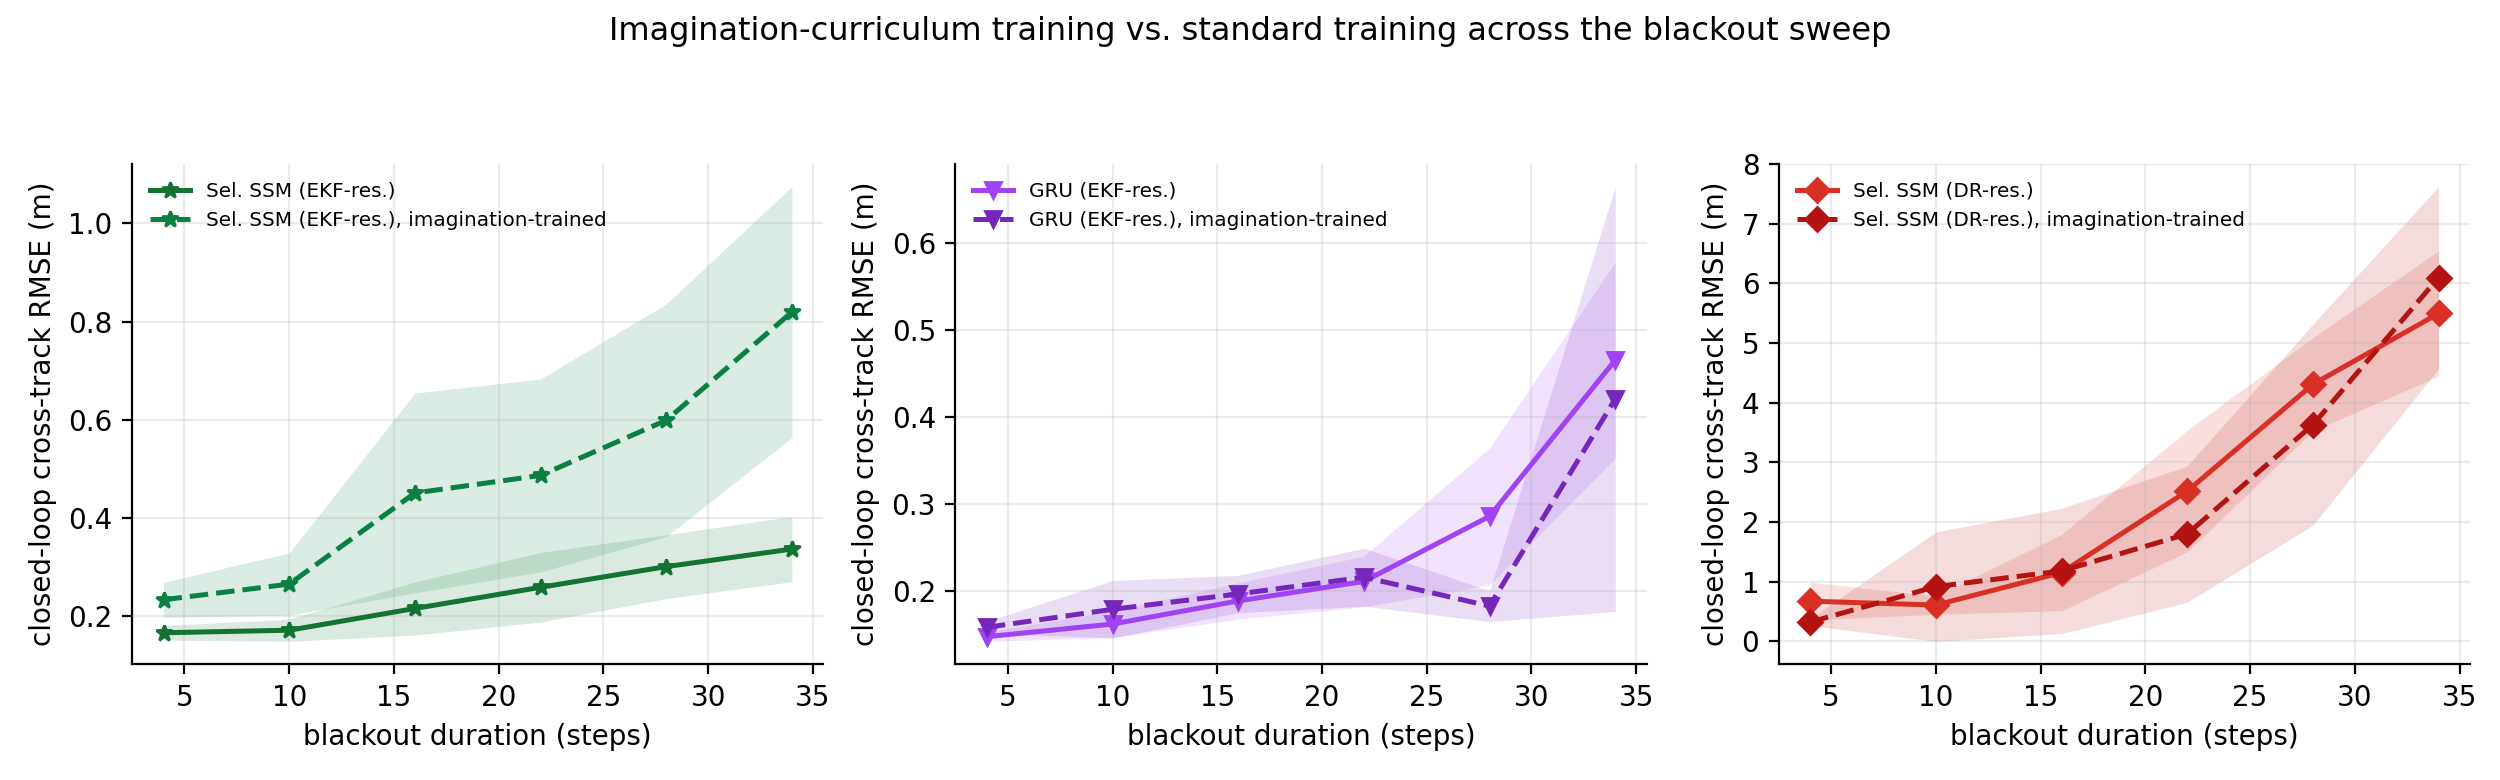
\includegraphics[width=0.94\linewidth]{figures/fig_dropout_curriculum.png}
\caption{Standard versus long-blackout training across the isolated blackout-duration sweep. GRU-EKF benefits only at the longest blackouts. SSM-EKF becomes worse across the sweep. SSM-DR shows no reliable gain.}
\label{fig:curriculum}
\end{figure}

The curriculum therefore does not act like a general robustness improvement. It can help a learned correction when the underlying state estimate is already well structured and several errors interact, but the same training distribution can move another architecture in the wrong direction. The result also rules out a simple explanation in which better exposure to long blind windows must improve performance during long blind windows.

\section{What this implies for robot world-model benchmarks}

The testbed is small, but the failure mode is general. A robot world model is rarely evaluated and deployed under exactly the same information pattern. An offline benchmark may ask for a long imagined future from a fixed context, while the deployed robot receives new camera frames, proprioception, force feedback, or language instructions and replans after a much shorter interval. The benchmark can then reward a capability that matters without measuring the mixture of prediction and correction that actually drives behavior.

\textbf{Evaluate the feedback schedule, not only the prediction horizon.} A horizon $H$ is incomplete without specifying what the model is allowed to observe before and during those $H$ steps. For a model used with frequent replanning, evaluation should include periodic reconditioning. For a model expected to run open loop, a blind rollout is appropriate. The evaluation protocol should mirror that choice rather than assume one setting is universally more faithful.

\textbf{Report decision-level agreement alongside fidelity.} Prediction metrics should be paired with a downstream quantity such as control regret, success-rate ranking, or policy-selection agreement. In our testbed, a metric with apparently more relevant temporal structure produces worse model selection. Measuring ranking agreement makes that failure visible even when average prediction errors look reasonable.

\textbf{Separate physical prediction from state correction.} Modern robot world models increasingly combine video, action, proprioception, and other modalities. New observations are not merely extra inputs; they change the role of the predictive model. A model that is excellent at extrapolation may be poor at incorporating corrections, and a model that drifts during a long blind rollout may still be useful when regularly grounded. Physical accuracy should therefore be evaluated both across imagined time and at the points where the model is reconnected to the real sensor stream.

These conclusions do not favor one-step metrics in general, and they do not argue against imagination-based learning. Systems such as Dreamer, DreamZero, or planning with video world models may spend much more time in imagined futures than the estimator in this paper. In those systems, multi-step fidelity may become more predictive. The point is that this relationship should be measured, not assumed.

\section{Limitations}

This study deliberately removes much of what makes current robot world models difficult. It uses a three-dimensional state rather than images or learned latent representations, a single simulated robot and reference path, and a fixed pure-pursuit controller. It does not test a learned action generator or a visual generative model. The primary long-blackout comparison uses one training seed per model, with three seeds only for SSM-EKF$^\dagger$. The blind-rollout metric uses a fixed horizon of $H=20$, and we do not sweep the frequency of reconditioning directly. The compound-stress result is one combined condition rather than a full factorial sweep. Physical MRCLAM logs are available in the broader project, but they do not constitute a hardware closed-loop experiment.

These limitations constrain the scope of the claim. The paper does not establish which metric should be used for large visual world models. It establishes a simpler point: even in a system where dynamics, sensing, and downstream behavior can all be measured exactly, a more rollout-like offline metric can be a worse predictor of control. A stronger follow-up should repeat the experiment while varying the observation/replanning interval and then move the same evaluation protocol to richer learned world models and hardware.

\section{Conclusion}

A world model is useful to a robot only through the decisions it supports. In this controlled tracking problem, a 20-step observation-free rollout is less predictive of closed-loop model choice than ordinary replay position error, even though the rollout looks more like imagination-based planning. Training on longer blind intervals also produces conditional rather than uniform gains: it helps EKF-anchored models under compound stress, but not every model or every blackout regime.

The practical lesson is to make feedback part of world-model evaluation. Measure how accurately a model predicts, but also specify when it will observe again, when it will be reconditioned, and how prediction error changes action. For robot learning, the most informative world-model benchmark is not the one with the longest rollout. It is the one that most closely matches the loop in which the model will actually be used.

\section*{Acknowledgments}
This project began as a final project for ECE~6562 (Autonomous Control of Robotic Systems), Georgia Institute of Technology, Summer 2026, and was extended with the blind-rollout evaluation and long-blackout training experiments reported here.

\bibliographystyle{plainnat}
\bibliography{references}

\appendix
\section{Seed robustness of the long-blackout training arm}
\label{app:seeds}

\begin{table}[h]
\centering
\small
\caption{SSM-EKF$^\dagger$ cross-track RMSE (m) across three independent training seeds. The model remains worse than the standard SSM-EKF at the long-blackout condition.}
\begin{tabular}{lccc}
\toprule
Condition & seed 0 & seed 1 & seed 2 \\
\midrule
Nominal             & 0.309 & 0.295 & 0.271 \\
Long blackout (34)  & 0.819 & 0.799 & 0.785 \\
High range noise    & 0.305 & 0.351 & 0.340 \\
Two landmarks       & 1.037 & 0.536 & 0.611 \\
High gyro bias      & 0.316 & 0.349 & 0.305 \\
\bottomrule
\end{tabular}
\end{table}

\section{Code and reproducibility}
All simulation, training, and evaluation code, bundled checkpoints, and raw result JSON files are included in the accompanying submission package. \texttt{reproduce\_worldmodel.sh} regenerates the paper tables and figures and can retrain the long-blackout models from scratch.

\end{document}
